\documentclass{article}
\usepackage[UTF8]{ctex}
\usepackage[T1]{fontenc}
\usepackage[utf8]{inputenc}
\usepackage{latexsym}
\usepackage{amsmath}
\usepackage{siunitx}
\usepackage{float}
\usepackage[table,xcdraw]{xcolor}
\usepackage{listings}
\usepackage{graphicx}
\usepackage{graphics}
\lstset{
    basicstyle = \ttfamily,
    keywordstyle = \bfseries,
    linewidth = \linewidth,
    xleftmargin=.2\textwidth,
    xrightmargin=.2\textwidth,
    numbers = left,
    numberstyle = \textcircled,
    frame = none,
}
\title{Homework 2}
\author{PB17000297 罗晏宸}
\date{March 20 2020}

\begin{document}
\maketitle

\section{}
使用以下代码段(假定 R3 的初值为 R2+396):

\begin{lstlisting}[language={[x86masm]Assembler}]
Loop:   LD      R1, 0(R2);
        DADDI   R1, R1, #1;
        SD      R1, 0, (R2);
        DADDI   R2, R2, #4;
        DSUB    R4, R3, R2;
        BNEZ    R4, Loop;
\end{lstlisting}
\subparagraph{a} 列出上述代码中的所有数据相关,需写出数据相关类型,并记录寄存器,源指令和目标指令。例如,从指令\textcircled{1}到指令\textcircled{2}存在对于寄存器 R1 的 RAW 相关。
\subparagraph{b} 给出这一指令序列对于 5 级 RISC 流水线的时序,该流水线没有设置任何旁路定向路径(Bypass or Forwarding),但假定在同一时钟周期中的寄存器读取与写入通过该寄存器堆进行“转发”,且分支是通过冲刷流水线来处理的。如果所有存储器引用耗时一个周期,这一循环的执行需要多少个周期?
\subparagraph{c} 给出这一指令序列对于拥有完整旁路定向路径的 5 级 RISC 流水线的时序。如果所有存储器引用耗时一个周期,且在处理分支时采用预测转移失败策略,这一循环的执行需要多少个周期?
\subparagraph{d} 给出这一指令序列对于拥有完整旁路定向路径的 5 级 RISC 流水线的时序。如果所有存储器引用耗时一个周期,且在处理分支时采用预测转移成功策略,这一循环的执行需要多少个周期?

\paragraph{解}
\subparagraph{a}
\begin{itemize}
    \item 从指令\textcircled{1}到指令\textcircled{2}存在对于寄存器 R1 的 RAW 相关。
    \item 从指令\textcircled{1}到指令\textcircled{2}存在对于寄存器 R1 的 WAW 相关。
    \item 从指令\textcircled{1}到指令\textcircled{3}存在对于寄存器 R1 的 RAW 相关。
    \item 从指令\textcircled{2}到指令\textcircled{3}存在对于寄存器 R1 的 WAW 相关。
    \item 从指令\textcircled{3}到指令\textcircled{4}存在对于寄存器 R1 的 WAR 相关。
    \item 从指令\textcircled{3}到指令\textcircled{4}存在对于寄存器 R2 的 WAR 相关。
    \item 从指令\textcircled{4}到指令\textcircled{5}存在对于寄存器 R2 的 RAW 相关。
    \item 从指令\textcircled{5}到指令\textcircled{6}存在对于寄存器 R4 的 RAW 相关。
\end{itemize}

\subparagraph{b}
R3初值为R2+396,每次循环都给R2加4,直到R2=R3时终止循环。一共要$396 \div 4 = 99$个周期。
根据题意,要解决所有的数据相关,需要在指令3,4,5,6的IF段后加入两个stall,停止两个周期来保证解决数据相关。时序为:

\begin{table}[H]
    \centering
    \resizebox{\columnwidth}{!}{
    \begin{tabular}{|l|c|c|c|c|c|c|c|c|c|c|c|c|c|c|c|c|c|c|c|}
    \hline
                      & 1  & 2  & 3  & 4                        & 5                        & 6  & 7                        & 8                        & 9  & 10 & 11                       & 12                       & 13 & 14                       & 15                       & 16                       & 17                       & 18 & 19 \\ \hline
    \texttt{Loop:~~~~LD  R1, 0(R2); } & IF & ID & EX & M                        & WB                       &    &                          &                          &    &    &                          &                          &    &                          &                          &                          &                          &    &    \\ \hline
    \texttt{~~~~~~~~DADDI R1, R1, \#1; } &    & IF & ID & {\color[HTML]{CB0000} S} & {\color[HTML]{CB0000} S} & EX & M                        & WB                       &    &    &                          &                          &    &                          &                          &                          &                          &    &    \\ \hline
    \texttt{~~~~~~~~SD R1, 0, (R2); }     &    &    & IF & {\color[HTML]{CB0000} S} & {\color[HTML]{CB0000} S} & ID & {\color[HTML]{CB0000} S} & {\color[HTML]{CB0000} S} & EX & M  & WB                       &                          &    &                          &                          &                          &                          &    &    \\ \hline
    \texttt{~~~~~~~~DADDI R2, R2, \#4; }  &    &    &    & {\color[HTML]{CB0000} S} & {\color[HTML]{CB0000} S} & IF & {\color[HTML]{CB0000} S} & {\color[HTML]{CB0000} S} & ID & EX & M                        & WB                       &    &                          &                          &                          &                          &    &    \\ \hline
    \texttt{~~~~~~~~DSUB R4, R3, R2; }    &    &    &    &                          &                          &    & {\color[HTML]{CB0000} S} & {\color[HTML]{CB0000} S} & IF & ID & {\color[HTML]{CB0000} S} & {\color[HTML]{CB0000} S} & EX & M                        & WB                       &                          &                          &    &    \\ \hline
    \texttt{~~~~~~~~BNEZ R4, Loop; }     &    &    &    &                          &                          &    &                          &                          &    & IF & {\color[HTML]{CB0000} S} & {\color[HTML]{CB0000} S} & ID & {\color[HTML]{CB0000} S} & {\color[HTML]{CB0000} S} & EX                       & M                        & WB &    \\ \hline
                      &    &    &    &                          &                          &    &                          &                          &    &    &                          &                          & IF & {\color[HTML]{CB0000} S} & {\color[HTML]{CB0000} S} & {\color[HTML]{CB0000} S} & {\color[HTML]{CB0000} S} & IF &    \\ \hline
    \end{tabular}
    }
\end{table}
循环需要17个时钟周期,因此总共的时钟周期数为
$$
    (99 - 1) \times 17 + (17 + 1) = 1684
$$
\subparagraph{c}
在有完整旁路时,使用预测转移失败策略,需要在BNEZ指令之后冲刷流水线,时序为:

\begin{table}[H]
    \centering
    \resizebox{\columnwidth}{!}{
    \begin{tabular}{|l|c|c|c|c|c|c|c|c|c|c|c|c|}
    \hline
                       & 1  & 2  & 3  & 4                        & 5                         & 6  & 7                         & 8                         & 9                           & 10                          & 11                        & 12                      \\ \hline
    \texttt{Loop:~~~LD R1, 0(R2);} & IF & ID & EX & M                        & WB                        &    &                           &                           &                             &                             &                           &                         \\ \hline
    \texttt{~~~~~~~~DADDI R1, R1, \#1;} &    & IF & ID & {\color[HTML]{CB0000} S} &  EX & M  & WB                        &                           &                             &                             &                           &                         \\ \hline
    \texttt{~~~~~~~~SD R1, 0, (R2);}    &    &    & IF & {\color[HTML]{CB0000} S} &  ID & EX &  M  &  WB &                             &                             &                           &                         \\ \hline
    \texttt{~~~~~~~~DADDI R2, R2, \#4;} &    &    &    & {\color[HTML]{CB0000} S} &  IF & ID &  EX &  M  & WB                          &                             &                           &                         \\ \hline
    \texttt{~~~~~~~~DSUB R4, R3, R2;}   &    &    &    &                          &                           & IF &  ID &  EX & M                           & WB                          & {\color[HTML]{CB0000} }   & {\color[HTML]{CB0000} } \\ \hline
    \texttt{~~~~~~~~BNEZ R4, Loop;}     &    &    &    &                          &                           &    & IF                        & ID                        & EX                          & M                           &  WB & {\color[HTML]{CB0000} } \\ \hline
    \texttt{~~~~~~~~LW R1, 0(R2);}      &    &    &    &                          &                           &    &                           & IF                        & {\color[HTML]{CB0000} Miss} & {\color[HTML]{CB0000} Miss} & IF                        &                         \\ \hline
    \end{tabular}
    }
\end{table}
循环需要10个时钟周期,因此总共的时钟周期数为
$$
    (99 - 1) \times 9 + (9 + 1) = 991
$$

\subparagraph{d}
在有完整旁路时,使用预测转移成功策略,不进行冲刷,时序为:

\begin{table}[H]
    \centering
    \resizebox{\columnwidth}{!}{
    \begin{tabular}{|l|c|c|c|c|c|c|c|c|c|c|c|c|c|}
    \hline
                       & 1  & 2  & 3  & 4                        & 5                         & 6  & 7                         & 8                         & 9                         & 10                        & 11                       & 12                        & 13 \\ \hline
    \texttt{Loop:~~~LD R1, 0(R2);} & IF & ID & EX & M                        & WB                        &    &                           &                           &                           &                           &                          &                           &    \\ \hline
    \texttt{~~~~~~~~DADDI R1, R1, \#1;} &    & IF & ID & {\color[HTML]{CB0000} S} &  EX & M  & WB                        &                           &                           &                           &                          &                           &    \\ \hline
    \texttt{~~~~~~~~SD R1, 0, (R2);}    &    &    & IF & {\color[HTML]{CB0000} S} &  ID & EX &  M &  WB &                           &                           &                          &                           &    \\ \hline
    \texttt{~~~~~~~~DADDI R2, R2, \#4;} &    &    &    & {\color[HTML]{CB0000} S} &  IF & ID &  EX &  M & WB                        &                           &                          &                           &    \\ \hline
    \texttt{~~~~~~~~DSUB R4, R3, R2;}   &    &    &    &                          &                           & IF &  ID &  EX & M                         & WB                        & {\color[HTML]{CB0000} }  & {\color[HTML]{CB0000} }   &    \\ \hline
    \texttt{~~~~~~~~BNEZ R4, Loop;}     &    &    &    &                          &                           &    & IF                        & {\color[HTML]{CB0000} S}  & ID                        & EX                        &  M &  WB &    \\ \hline
                       &    &    &    &                          &                           &    &                           & & IF                        &  ID &  EX & M                        &                            \\ \hline
    \end{tabular}
    }
\end{table}
循环需要9个时钟周期,因此总共的时钟周期数为
$$
    (99 - 1) \times 8 + 12 = 796
$$

\section{}
有一条静态多功能流水线由 5 段组成,加法用 1,3,4,5 段,乘法用 1,2,5 段,第三段的时间为$2\Delta t$ ,其余各段时间均为$\Delta t$ ,而且流水线的输出可以直接返回输入端或暂存于相应的流水寄存器中。现要在该流水线上计算$\displaystyle \prod_{i = 1}^4(A_i + B_i)$,画出其时空图,并计算其吞吐率、加速比和效率。
\begin{figure}[H]
    \centering
    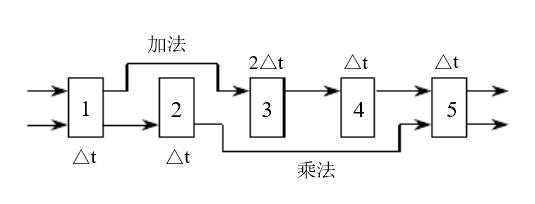
\includegraphics[width = 270pt]{2.jpg}
\end{figure}

\paragraph{解}
首先计算四次加法$A_i + B_i$,再计算两次乘法$(A_i + B_i) \times (A_{i + 1} + B_{i + 1})$,再对结果做一次乘法,时空图如下:

\begin{table}[H]
    \centering
    \resizebox{\columnwidth}{!}{
        \begin{tabular}{|c|c|c|c|c|c|c|c|c|c|c|c|c|c|c|c|c|c|c|c|}
            \hline
            5 &                          &                          &                          &                          & \cellcolor[HTML]{FD6864} &                          & \cellcolor[HTML]{FE0000} &                          & \cellcolor[HTML]{CB0000} &                          & \cellcolor[HTML]{9A0000} &                          &                          & \cellcolor[HTML]{3166FF} & \cellcolor[HTML]{3531FF} &                          &                          & \cellcolor[HTML]{00009B} &    \\ \hline
            4 &                          &                          &                          & \cellcolor[HTML]{FD6864} &                          & \cellcolor[HTML]{FE0000} &                          & \cellcolor[HTML]{CB0000} &                          & \cellcolor[HTML]{9A0000} &                          &                          &                          &                          &                          &                          &                          &                          &    \\ \hline
            3 &                          & \cellcolor[HTML]{FD6864} & \cellcolor[HTML]{FD6864} & \cellcolor[HTML]{FE0000} & \cellcolor[HTML]{FE0000} & \cellcolor[HTML]{CB0000} & \cellcolor[HTML]{CB0000} & \cellcolor[HTML]{9A0000} & \cellcolor[HTML]{9A0000} &                          &                          &                          &                          &                          &                          &                          &                          &                          &    \\ \hline
            2 &                          &                          &                          &                          &                          &                          &                          &                          &                          &                          &                          &                          & \cellcolor[HTML]{3166FF} & \cellcolor[HTML]{3531FF} &                          &                          & \cellcolor[HTML]{00009B} &                          &    \\ \hline
            1 & \cellcolor[HTML]{FD6864} &                          & \cellcolor[HTML]{FE0000} &                          & \cellcolor[HTML]{CB0000} &                          & \cellcolor[HTML]{9A0000} &                          &                          &                          &                          & \cellcolor[HTML]{3166FF} & \cellcolor[HTML]{3531FF} &                          &                          & \cellcolor[HTML]{00009B} &                          &                          &    \\ \hline
              & 1                        & 2                        & 3                        & 4                        & 5                        & 6                        & 7                        & 8                        & 9                        & 10                       & 11                       & 12                       & 13                       & 14                       & 15                       & 16                       & 17                       & 18                       & 19 \\ \hline
            \end{tabular}
    }
\end{table}
在$18\Delta t$的时间中,得到7个结果,吞吐率为
\begin{equation*}
    \text{TP} = \frac{7}{18\Delta t}
\end{equation*}

加速比为:
\begin{equation*}
    \text{S} = \frac{5 \times 4\Delta t + 3 \times 3 \Delta t}{18 \Delta t} = \frac{29}{18} \approx 1.611
\end{equation*}

效率为:
\begin{equation*}
    \text{E} = \frac{5 \times 4\Delta t + 3 \times 3\Delta t}{5 \times 18\Delta t} = \frac{29}{90} \approx 0.322
\end{equation*}


\section{}
假定原机器是一个 5 级流水线,其时钟周期为 \SI{1}{\nano\second}。第二种机器为 12 级流水线,时钟周期为 \SI{0.6}{\nano\second}。由于数据相关,5 级流水线每 5 条指令经历一次 stall,而 12 级流水线每 8 条指令经历三次 stall。此外,分支占全部指令的 20\%,两台机器的预测错误率都是 5\%。
\subparagraph{a} 仅考虑数据相关,12 级流水线相对于 5 级流水线的加速比为多少?
\subparagraph{b} 在考虑分支预测错误而导致 stall 的情况下,如果第一台机器的分支预测错误的额外代价为 2 个周期,而第二台机器为 5 个周期,则每种机器的 CPI 为多少?

\paragraph{解}
\subparagraph{a}
仅考虑数据相关,加速比为:
\begin{equation*}
    \text{S} = \frac{\frac{8 \times 12 + 3}{8} \times 0.6}{\frac{5 \times 5 + 1}{5} \times 1} = \frac{297}{208} \approx 1.428
\end{equation*}

\subparagraph{b}
第一台机器:
\begin{equation*}
    \text{CPI} = 5 + \frac{1}{5} + 2 \times 0.2 \times 0.05 = 5.22
\end{equation*}

第二台机器:
\begin{equation*}
    \text{CPI} = 12 + \frac{3}{8} + 2 \times 0.2 \times 0.05 = 12.395
\end{equation*}
\end{document}